
\section{Continuous interior penalty methods for the biharmonic problem with Cahn-Hilliard type boundary conditions}%
\label{sec:CIP_biharmonic_problem}

One of the objective of this section is to discuss the strong formulation for the biharmonic problem.
Following this, we will present both the continuous weak formulation and the derivation of the two proposed discrete weak formulations, specifically the continuous interior penalty methods.
We then present a short discussion of the current status of the properties of the methods.

\subsection{The biharmonic problem with C-H boundary conditions}%
\label{sub:the_biharmonic_problem_with_c_h_boundary_conditions}

Let $\Omega \subseteq    \mathbb{R} ^d$ be a bounded polygonal domain and $\Gamma $ be its corresponding boundary. Also let $\mathcal{T}_{h} = \left\{ T \right\} $ be a shape-regular fitted mesh s.t. $\mathcal{T}_{h} = \Omega $. Let the biharmonic problem have the form,
\begin{subequations}
\begin{align}
    \Delta^2  u  + \alpha  u  & = f( x)  \quad \text{in } \Omega,   \label{eq:bi_problem_a}\\
    \partial _{n} u & = g_{1}(x)   \quad \text{on } \Gamma ,  \label{eq:bi_problem_b}\\
    \partial _{n} \Delta  u & = g_{2}( x)   \quad \text{on } \Gamma .  \label{eq:bi_problem_c}
\end{align}
\label{eq:bi_problem}
\end{subequations}
Here is $\Delta ^2 = \Delta  \left( \Delta  \right) $ the biharmonic operator, also known as the bilaplacian. We will assume for the strong form that $u \in H^{4}\left( \Omega  \right) $, $\alpha  >0 $ and $f \in L^{2}\left( \Omega  \right)
$. The functions $g_{1},g_{2}: \Omega  \to \mathbb{R}$ are denoted as boundary conditions similar to the CH problem.

\begin{remark}
It is worth noting that the problem is closely related to the Kirchhoff's plate problem by changing the boundary conditions such that $u = \partial _{n } u = 0$ on $\Gamma $, which is in the literature known as so-called clamped boundary conditions.
Many of the papers we refer to may consider clamped boundary condition and not the CH boundary conditions. The main difference relies on if the problem is treated with homogeneous or non-homogeneous boundary conditions and if the discrete space is
imposing the Dirichlet and Neumann conditions strongly in the discrete solution space or weakly using the Nitsche's method \cite{nitsche1971variationsprinzip}.
\end{remark}

We want to construct a weak form for the strong biharmonic problem \eqref{eq:bi_problem}. Let $v \in H^{2}( \Omega ) $  Using Greens Theorem is it obvious that \(
\left( \Delta ^2 u,v \right) _{ \Omega  }   = ( \partial _{n} \Delta u, v ) _{\Gamma   } - ( \nabla \left( \Delta  u \right) , \nabla v ) _{ \Omega }
\).
Next, applying a new iteration of the Greens theorem we get
$ -( \nabla ( \Delta u ) , \nabla v ) _{\Omega  }  =   ( \Delta u, \Delta v ) _{\Omega } - ( \Delta u, \partial _{n}v )_{\Gamma } $.
Hence, we obtain the identity
\begin{equation}
\label{eq:iden_bi}
( \Delta ^2 u, v ) _{\Omega } = ( \Delta u, \Delta v)_{\Omega } +  ( \partial _{n} \Delta u, v)_{\Gamma } - ( \partial _{n} v, \Delta u) _{\Gamma }
\end{equation}
Taking into account the boundary conditions, we end up with the following corresponding weak formulation of the biharmonic problem \eqref{eq:bi_problem}.

\begin{equation}
\label{eq:V_deg}
V := \left\{ v \in  H^s( \Omega ), \  s \ge  5  /2 + \varepsilon   \mid \partial _{n} v  = g_{1}     \right\}
\end{equation}
Consider the bilinear form $a:V\times V \to \mathbb{R}$ and the linear form $l: V \to \mathbb{R}$. We define the continuous weak formulation problem formulation as follows.


\begin{equation}
\label{eq:cont_weak_problem}
\text{Find } u \in V   \text{ such that } a( u,v) = l( v)  \forall v \in V
\end{equation}
where
\begin{equation}
    \begin{split}
a( u,v) & =  ( \alpha u,v)_{\Omega } + ( \Delta u, \Delta v)_{\Omega } - (  \Delta u, \partial _{n} v) _{\Gamma }\\
l( v)  &= ( f,v)_{\Omega } - ( g_{2} , v)_\Omega
    \end{split}
\end{equation}
Note that the Neumann boundary condition $g_{1}$ is strongly imposed in $V$, and $g_{2}$ is naturally incorporated in the weak formulation.


\subsection{Detailed construction of Hessian and Laplacian Formulations }%
\label{sub:construction_of_laplacian_cip}
The goal is to construct two CIP formulations for the problem \eqref{eq:cont_weak_problem}, that is: Find $u_{h} \in V_{h} \not\in V$ such that $a_{h}( u_{h}, v_{h}) = l_{h}( v_{h}) $ for all $v_{h} \in V_{h}$. We will follow the ideas presented in \cite{brenner2012} and \cite{feng2007fully}.
A property that is necessary is that when we have a bilinear form and replace the exact solution with $u_{h} \in V_{h}$, the system still remains consistent in $V$. Hence, we guarantee a consistency of the discrete weak formulation by assuming during
the construction that $u \in H^{4}( \Omega ) $ and $v_{h} \in  V_{h}$ .
 However, due to the nonconformal nature of $V_{h}$, it becomes necessary to introduce penalty terms to ensure the discrete system is well-posed when we replace with $u_{h} \in V_{h}$. Keep in mind that the $C^{1}$
continuity is imposed weakly and in the same way is the Neumann conditions also imposed weakly.

To achieve the objective of constructing the Hessian and Laplacian formulations, the following lemmas will be the primary components.

\subsubsection{Construction of the Hessian formulation}%
\label{ssub:construction_of_the_hessian_formulation}



\begin{lemma}
    \label{lemma:hessian}
    Assume the homogeneous Neumann conditions $g_1 = 0 $.
Let $u \in H^{4}( \Omega ) $ be the solution to \eqref{eq:bi_problem}, let $ v_{h} \in V_{h}$ and a constant $\gamma >0$. Then does the following identity hold.
\begin{equation}
\label{eq:bi_basic_dg_full}
\begin{split}
    \left( \Delta  ^{2} u, v_h \right) _{\Omega }  =&   \left( D^2u, D^2v_h \right)_{\Omega } +  \left(g_{2}, v_h  \right) _{ \Gamma  }\\
    &    -  ( \mean{ \partial _{nn} u }   , \jump{ \partial_{n} v_h } )_{\mathcal{F}_{h}^{int} } -  (  \jump{ \partial_{n} u
    },\mean{ \partial _{nn} v_h } )_{\mathcal{F}_{h}^{int} } + \frac{\gamma }{h} (  \jump{ \partial_{n} u
    },\mean{ \partial _{nn} v_h } )_{\mathcal{F}_{h}^{int} } \\
    & - ( \partial _{nn} u , \partial _{n} v_h)_{\Gamma  }- ( \partial _{n} u , \partial _{nn} v_h)_{\Gamma  } + \frac{\gamma }{h}  \left(  \partial _{n} u,  \partial _{n} v_{h}      \right)_{\Gamma }
\end{split}
\end{equation}
\end{lemma}


\begin{figure}[h]
\centering
    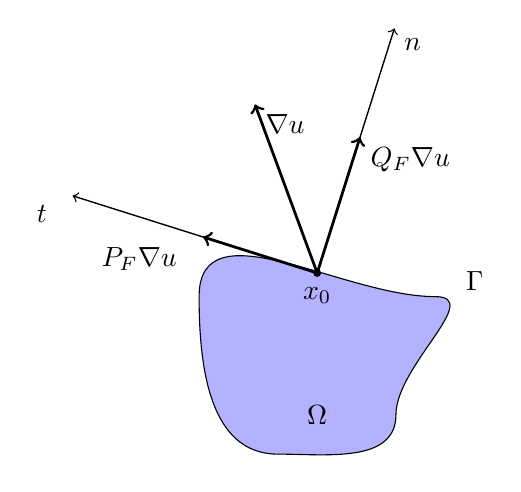
\begin{tikzpicture}
        % Define points for square
        \coordinate (A) at (-0.5,-0.5);
        \coordinate (B) at (1.0,0.0);
        \coordinate (C) at (1.5,1.5);
        \coordinate (D) at (-1.5,1.5);
        \filldraw[fill=blue!30,draw=black] (A) to[out=0,in=-90] (B) to[out=90,in=0] (C) to[out=180,in=90] (D) to[out=-90,in=180] cycle;


        \def\lenfactorn{4.5} % change this value to easily adjust the length of n
        \def\lenfactort{4.5} % change this value to easily adjust the length of t
        \draw[->, line width=0.5pt] ({1.8*cos(90)}, {1.8*sin(90)}) -- ({1.8*cos(90) + \lenfactorn*(2.5*cos(85) - 1.8*cos(90))}, {1.8*sin(90) + \lenfactorn*(2.5*sin(85) - 1.8*sin(90))}) node[below right, xshift=-0.0cm] {$n $};
        \draw[->, line width=0.5pt, rotate around={90:({1.8*cos(90)}, {1.8*sin(90)})}] ({1.8*cos(90)}, {1.8*sin(90)}) -- ({1.8*cos(90) + \lenfactort*(2.5*cos(85) - 1.8*cos(90))}, {1.8*sin(90) + \lenfactort*(2.5*sin(85) - 1.8*sin(90))}) node[below left, xshift=-0.2cm] {$t $};

        \def\lenfactorPf{2.5} % change this value to easily adjust the length of Pf
        \def\lenfactorQf{2.1} % change this value to easily adjust the length of Qf
        \draw[->, line width=1.0pt] ({1.8*cos(90)}, {1.8*sin(90)}) -- ({1.8*cos(90) + \lenfactorPf*(2.5*cos(85) - 1.8*cos(90))}, {1.8*sin(90) + \lenfactorPf*(2.5*sin(85) - 1.8*sin(90))}) node[below right, xshift=-0.0cm] {$Q_F\nabla u$};
        \draw[->, line width=1.0pt, rotate around={90:({1.8*cos(90)}, {1.8*sin(90)})}] ({1.8*cos(90)}, {1.8*sin(90)}) -- ({1.8*cos(90) + \lenfactorQf*(2.5*cos(85) - 1.8*cos(90))}, {1.8*sin(90) + \lenfactorQf*(2.5*sin(85) - 1.8*sin(90))}) node[below left, xshift=-0.2cm] {$P_F\nabla u$};
        \def\lenfactorGradu{1.3} % change this value to easily adjust the length of \nabla u
        \draw[->, line width=1.0pt] ({1.8*cos(90)}, {1.8*sin(90)}) -- ({1.8*cos(90) + \lenfactorGradu*(3.5*cos(100) - 1.8*cos(90))}, {1.8*sin(90) + \lenfactorGradu*(3.5*sin(100) - 1.8*sin(90))}) node[below right, xshift=-0.0cm] {$\nabla u$};

        \node[circle,fill,inner sep=1pt,label={below:$x_0$}] at ({1.8*cos(90)}, {1.8*sin(90)}) {};
        \node at (0,0) {$\Omega$};
        \node at (2,1.7) {$\Gamma$};

    \end{tikzpicture}
\caption{Let $x_{0}$ be a point at the boundary $\Gamma $ for dimension $d=2$. Here is a illustration of the gradient $\nabla u$ with the corresponding normal and tangential decomposition, $Q_{F} \nabla  u$ and $P_{F} \nabla  u$.    }
\label{fig:projection_QF_PF}
\end{figure}
\begin{proof}

 We will start constructing a local theory for a element $T$ and then extend it to the full mesh
$\mathcal{T}_{h} $. Using Greens Theorem is it obvious that
\begin{equation}
    \label{eq:id1}
\left( \Delta ^2 u,v_h \right) _{T }   = \left( \partial _{n} \Delta u, v_h \right) _{\partial T  } - \left( \nabla \left( \Delta  u \right) , \nabla v_h \right) _{T }
\end{equation}

We can expand the second term in the following way.
\begin{equation}
    \label{eq:id2}
    \begin{split}
( \nabla ( \Delta u ) , \nabla v_h ) _{T } & = \sum_{i = 1}^{ d}  ( \Delta  \partial _{x_{i}} u, \partial _{x_{i}}v_h ) _{T }
                                           = \sum_{i = 1}^{d}  ( \nabla \cdot ( \nabla \partial _{x_{i}} u ) , \partial _{x_{i}} v_h )_{T }  \\
&= \sum_{i = 1}^{d}  \left( ( \partial_n  \partial _{x_{i}} u,  \partial _{x_{i}} v_h ) _{\partial T } -   ( \nabla \partial _{x_{i}} u, \nabla \partial _{x_{i}} v_h )_{T } \right) \\
& = (  \partial_n\nabla u, \nabla v_h ) _{\partial_{} T  } - ( D^2 u, D^2v_h ) _{T }
    \end{split}
.\end{equation}
Hence, the normal flux of $\Delta u$ appears naturally into the formulation. It can be denoted that $D^2$ is the Hessian matrix operator. Also remark that we apply the notation
$( D^2u, D^2v_h )_{\Omega } = \int_{\Omega }^{} D^{2}u : D^2v_h  dx$ for the inner product $D^2u:D^2v_h$.

Next, we want to decompose the evaluation of $\nabla  u $ on the boundary $\partial T$ in the tangential and normal direction. Pick a facet  $F \in \partial T$, then we define the following decomposition of linear transformation $\nabla u = P_{F}\nabla u  + Q_{F}  \nabla u  $ s.t. the
orthogonality, $
P_{F} \nabla u  \cdot Q_{F}  \nabla u = 0$, holds. Here, the normal projection matrix is defined as $Q_{F} = n \otimes n $ and the tangential decomposition follows from $ P_{F} = I - Q_{F} = I - n \otimes n  =  \sum_{i=1}^{d-1} t_{i} \otimes t_i$,
where we defined a orthonormal basis $t_{i}$, $i = 1, \ldots, d-1$ for the space orthogonal to the outer normal vector $n$ on a facet $F$. For demonstration in $d=2$, see Figure \ref{fig:projection_QF_PF}. Let $ a_{1}, a_{2}, a_{3} \in \mathbb{R} ^{d}$ be any vectors, then it is well known that the following identity holds $ ( a_{1}
\otimes a_{2}  ) a_{3} = ( a_{2}^{T}  a_{3}) a_{1} $. Hence, we have
\begin{equation}
\label{eq:projection}
    \begin{split}
   Q_{F} \nabla u & = ( n \otimes n ) \nabla u =  (n^{T} \nabla u)n \\
   P_{F} \nabla u & =( I - n \otimes n ) \nabla u =   \nabla u  - (n^{T}  \nabla u)n =  \sum_{ i =1 }^{d-1} ( t_{i}^{T}  \nabla u ) t_{i}
    \end{split}
\end{equation}

Given that $u$ is evaluated only on $\partial T$ can we write
$\nabla u = \left( n^{T} \nabla u   \right) n + \sum_i^{d-1} \left( t_i^{T} \nabla u   \right) t_i$ such that,
\begin{equation}
\label{eq:id3}
    \begin{split}
(  \partial_n\nabla u, \nabla v_h ) _{\partial_{} T  } & =  ( \partial _{n} ( \partial_{n}u \ n), \partial _{n} v_h \ n )_{\partial T}   +\sum_{i,j=1}^{d-1} ( \partial _{n} ( \partial_{t_{i}}u \ t_{i}), \partial _{t_{j}} v_h \ t_{j} )_{\partial T} \\
& =  ( \partial _{nn} u, \partial _{n} v_h  )_{\partial T}+\sum_{i=1}^{d-1} ( \partial _{n t_{i}}u , \partial _{t_{i}} v_h  )_{\partial T}
    \end{split}
\end{equation}
Here we used that $n^{T} n = 1$ and $t_{i}^{T} t_{j} = \delta_{ij}$.
Remark that simple relation was applied,
    \begin{align*}
\partial_n (\partial_n u)  & = n^T \nabla (\partial_n u)  = n ^T (D^2 u \ n)  = n^{T} D^2 u \ n = \partial _{nn} u, \\
\partial_n (\partial_{t_{i}} u)  & = t_{i}^T \nabla (\partial_n u)  = t_i^T (D^2 u \ n )   = n^{T} D^2 u \ t_{i} = \partial _{n t_{i}} u.
    \end{align*}
We may also deduce the relationship $\partial _{nt_{i}} u = \partial _{t_{i}n}u$ which arise from the fact that $n^{T} D^2u \ t_{i} = ( t_{i}^{T} D^2u \  n)^T = t_{i}^{T}  D^2u \  n$, where we utilized the symmetry $D^2u = ( D^2u) ^{T} $ and that the
product is a scalar.
Combining \eqref{eq:id1}, \eqref{eq:id2} and \eqref{eq:id3} we see that,
\[
    ( \Delta ^2 u, v_h) _{T}   = ( D^2 u, D^2v_h)_{T } + ( \partial _{n}  \Delta u, v_h )_{\partial T} -( \partial _{nn}u , \partial _{n} v_h  )_{\partial T}-\sum_{i=1}^{d-1} ( \partial _{n t_{i}}u, \partial _{t_{i}} v_h  )_{\partial T}
\]
Since we aim construct a identity for the full mesh $\mathcal{T} _{h}$, we sum over the elements.
\begin{equation}
\label{eq:bi_basic_dg2}
\left( \Delta  ^{2} u,v_h \right) _{\Omega } = \sum_{T \in  \mathcal{T} _{h}}^{}  ( D^2 u, D^2v_h)_{T } + ( \partial _{n}  \Delta u, v_h )_{\partial T} -( \partial _{nn}u , \partial _{n} v_h  )_{\partial T}-\sum_{i=1}^{d-1} ( \partial _{n t_{i}} u , \partial _{t_{i}} v_h  )_{\partial T}
\end{equation}
Our goal is to simplify the equation above so we can take account for discontinuities of the derivatives.
By integrating over exterior facets $\mathcal{F} _{h}^{ext}$ and interior facets $\mathcal{F} _{h}^{int}$ we will get e more suitable formulation which makes it easier to control the jumps between the elements, hence makes it possible to penalize discontinuities.

\begin{equation*}
    \begin{split}
 ( \Delta  ^{2} u,v_h ) _{\Omega }  =&\sum_{T\in \mathcal{T} _{h}}^{} ( D^2u,D^2v_h ) _{T }  + (\partial _{n} \Delta  u,v_h)_{\partial T} - (\partial _{nn} u, \partial _{n}v_h )_{\partial T}  - \sum_{i=1}^{d-1} ( \partial _{t_{i}n}u , \partial _{t_{i}} v_h  )_{\partial T}   \\
= &\sum_{T\in \mathcal{T} _{h}}^{} ( D^2u,D^2v_h ) _{T }  + \sum_{F \in \mathcal{F}_{h}^{ext} }^{}  (\partial _{n} \Delta  u,v_h)_{F} - (\partial _{nn} u, \partial _{n}v_h )_{F}  - \sum_{i=1}^{d-1} ( \partial _{ t_{i}n} u , \partial _{t_{i}} v_h
)_{F}     \\
   &  + \sum_{F \in \mathcal{F} _{h}^{int}}^{} \underbrace{\left( (\partial _{n^{+}} \Delta  u^{+}
        ,v_h^{+} )_{F}
+ \left(\partial _{n^{-}} \Delta  u^{+} ,v_h^{-}\right)_{F}  \right)}_{(I)}    \\
    &\quad \quad  -
\underbrace{\left( \left(\partial _{n^{+}n^{+}} u^{+}, \partial _{n^{+}} v_h^{+} \right) _{F} + \left(\partial _{n^{-}n^{-}} u^{-}, \partial _{n^{-}} v_h^{-}
\right) _{F} \right) }_{(II)} \\
   &  \quad \quad - \sum_{i=1}^{d-1}\underbrace{( (\partial _{n^{+}t_{i}} u^{+}, \partial_{t_{i}} v_h^{+} )_{F} +  \left(\partial _{n^{-}t_{i}} u^{-},
        \partial_{t_{i}} v_h^{-}
\right)_{F} ) }_{(III)} \\
    \end{split}
.\end{equation*}

Where integration of the interior facets is computed in the following fashion.
\begin{equation}
    \label{eq:dg2_facets}
    \begin{split}
        (I) &  =    \left(\partial _{n^{+}} \Delta  u^{+} ,v_h^{+}\right)_{F} +
        \left(\partial _{n^{-}} \Delta  u^{-} ,v_h^{-}\right)_{F}  \\
            & =   \int_{F}^{}
            \jump{ \partial _{n} \Delta  u \cdot v_h } =
            \int_{F}^{}
            \mean{ \partial _{n} \Delta  u } \underbrace{\jump{ v_h }}_{= 0}    + \underbrace{\jump{ \partial _{n} \Delta  u
            }}_{= 0}    \mean{ v_h } = 0 \\
            (II) &  =     \left(\partial _{n^{+}n^{+}} u^{+}, \partial_{n^{+}} v_h^{+} \right)_{F} +  \left(\partial _{n^{-}n^{-}} u^{-}, \partial_{n^{-}} v_h^{-} \right)_{F}    \\
                 &= \int_{F}^{} \jump{ \partial _{nn} u \cdot  \partial_{n} v_h }   = \int_{F}^{}
                       \mean{ \partial _{nn} u    } \underbrace{\jump{ \partial_{n} v_h }  }_{\neq 0}    + \underbrace{\jump{ \partial
                               _{nn}  u
                       }}_{= 0}    \mean{ \partial _{n}v_h } \\
            (III) &  =     \left(\partial _{n^{+}t_{i}} u^{+}, \partial_{t_{i}} v_h^{+}
                \right)_{F} +  \left(\partial _{n^{-}t_{i}} u^{-}, \partial_{t_{i}} v_h^{-}
                \right)_{F}   \\
                 &  =   \int_{F}^{}
                 \jump{ \partial _{nt_{i}} u \cdot  \partial_{t_{i}} v_h } =
                 \int_{F}^{}
                 \mean{ \partial _{nt_{i}} u    } \underbrace{\jump{ \partial_{t_{i}} v_h }  }_{= 0}    + \underbrace{\jump{ \partial
                         _{nt_{i}}  u
                 }}_{= 0}    \mean{ \partial _{t_{i}}v_h }  = 0
                   \end{split}
.\end{equation}
Observe that the cancellations in the term $(I)$ and term $(III)$  appears of the continuity of $v_h\in V_{h} $ and $u\in H^{4}( \Omega ) $ which makes the jumps and derivative jumps zero. On the other hand, the second term $(II)$  does not vanish
since the derivative of $v_h \in V_{h}$ has a nonzero jump. It can also be raised that $\mean{
\partial _{nn} u } = \partial _{nn} u  $ holds of $H^{4}( \Omega  ) $.

Combining \eqref{eq:dg2_facets} and inserting the boundary condition $g_{2} = \partial _{n} \Delta u $ is it clear that the formulation presented in \eqref{eq:bi_basic_dg2} is equivalent to the following formulation.
\begin{equation}
\label{eq:bi_basic_dg_full_1}
\begin{split}
    \left( \Delta  ^{2} u, v_h \right) _{\Omega }  =&   \left( D^2u, D^2v_h \right)_{\mathcal{T} _{h}} +  \left(g_{2}, v_h  \right) _{\Gamma  }  -  ( \mean{ \partial _{nn} u }   , \jump{ \partial_{n} v_h } )_{\mathcal{F}_{h}^{int} } \\
                                                  &  - ( \partial _{nn} u , \partial _{n} v_h)_{\mathcal{F}^{ext}_{h} } - \sum_{i =1  }^{d-1} ( \partial   _{t_{i}n} u  ,  \partial   _{t_{i}}  v_h  )_{ \mathcal{F}^{ext} _{h}  }
\end{split}
\end{equation}
Under the assumption that $g_{1} = 0$ on $\Gamma$, and given that the tangential decomposition is orthogonal to $n$, we can assert that $ \partial_{t_{i} n} u = \partial_{t_{i}} ( \partial _{n} u )= \partial_{t_{i}} ( g_{1} ) = 0 $ holds for any $i =
1,\ldots, d -1$. This implies that the
last term of the equation vanish.

We also note that we add consistent symmetry terms $( \mean{ \partial _{nn} v_h } ,\jump{ \partial _{n} u }    )_{\mathcal{F}^{int}_{h} } $ and $( \partial _{nn} v_h  , \partial _{n} u     )_{\Gamma  } $ in addition to the penalty terms $\frac{\gamma
}{h} ( \partial _{n} u, \partial _{n}v)_{\Gamma }  $ and $\frac{\gamma
}{h} ( \jump{ \partial _{n} u }  , \jump{    \partial _{n}v})_{\mathcal{F}^{int}_{h} }  $ . Since $u\in H^{4}( \Omega ) $ and the boundary condition,  $\partial _{n} u = g_{1}=0$ on $\Gamma $, is each of these terms effectively zero, but does provide symmetry and will later
be proven to be essential for well-posedness for the discrete problem. Finally, we have
\begin{equation}
\begin{split}
    \left( \Delta  ^{2} u, v_h \right) _{\Omega }  =&   \left( D^2u, D^2v_h \right)_{\Omega } + \left(g_{2}, v_h  \right) _{ \Gamma  }\\
    &    -  ( \mean{ \partial _{nn} u }   , \jump{ \partial_{n} v_h } )_{\mathcal{F}_{h}^{int} } -  (  \jump{ \partial_{n} u
    },\mean{ \partial _{nn} v_h } )_{\mathcal{F}_{h}^{int} } + \frac{\gamma }{h}  (  \jump{ \partial_{n} u },\jump{ \partial _{n} v_h } )_{\mathcal{F}_{h}^{int} } \\
    & - ( \partial _{nn} u , \partial _{n} v_h)_{\Gamma  } - (\partial _{n} u, \partial _{nn} v_h )_{\Gamma  }  + \frac{\gamma }{h}  \left(  \partial _{n} u,  \partial _{n} v      \right)_{\Gamma }
\end{split}
\end{equation}

The proof is complete.

\end{proof}

Note that since $V_{h} \not\subset V $ is it necessary to define the space $V \oplus V_{h}$, which essentially is the direct sum of these two spaces. This new space includes all elements from $V$ and $V_h$ and all possible linear combinations of these elements. i.e., let $u \in V$ and $u_{h} \in V_{h}$, then $u + u_{h} \in V \oplus V_{h} $.

We will now assemble the Hessian CIP formulation.
Assume that the homogeneous boundary condition $g_{1}=0$.
The discrete problem is as follows:
 \begin{equation}
    \label{eq:hessian_prob}
    \text{Find } u_{h} \in V_{h} \text{ such that } a^{H}( u_{h}, v_{h})  = l_{h}^{H}( v_{h} )  \quad \forall v_{h} \in  V_{h}.
\end{equation}
Here is the corresponding bilinear and linear form  defined as,
\begin{equation}
    \label{eq:hessian_form}
\begin{split}
a_{h}^{H} \left( u_{h}, v_{h} \right)   =&
    \left( \alpha  u_{h}, v_{h} \right) _{\Omega }   +  \left( D^2 u_{h}, D^2v_{h} \right) _{\Omega } \\
 & - \left( \mean{  \partial _{n n} u_{h} }, \jump{ \partial _{n }v_{h}} \right)_{\mathcal{F}_{h}^{int}}  -
 \left( \jump{ \partial _{n}u_{h} }, \mean{ \partial _{n n} v_{h} } \right)_{\mathcal{F}_{h}^{int}}  + \frac{\gamma }{h}  \left( \jump{ \partial _{n} u_{h}}, \jump{ \partial _{n} v_{h}   }   \right)_{\mathcal{F}_{h}^{int}} \\
 & - \left(   \partial _{n n} u_{h} ,  \partial _{n }v_{h} \right)_{\Gamma }  -
 \left( \partial _{n}u_{h} , \partial _{n n} v_{h}       \right)_{\Gamma }  + \frac{\gamma }{h}  \left(  \partial _{n} u_{h},  \partial _{n} v_{h}      \right)_{\Gamma }   \\
 l_{h}^{H}( v_{h})  =&  \left( f, v_{h} \right) _{\Omega }  - \left(g_{2}, v_{h}  \right) _{\Gamma }
\end{split}
.
\end{equation}

With the corresponding energy norms,
\begin{equation}
\label{eq:a_cip_energy_norm_hes}
    \begin{split}
 \| v_{h} \|_{ a_{h}^{H} }^{ 2 }& = \alpha  \| v_{h}\|_{ \Omega  }^{2  }  +  \| D ^2 v_{h} \|_{ \Omega   }^{ 2 }  + \|  h^{-\frac{1}{2}} \jump{ \partial _{n} v_{h}    }\|_{  \mathcal{F} _{h}^{int} }^{2  }+ \|  h^{-\frac{1}{2}}  \partial _{n} v_{h}
 \|_{  \Gamma  }^{2  },  \quad v_{h} \in V_{h}  \\
   \| v \|_{ a_{h}^{H},* }^{ 2 } &= \| v \|_{ a_{h} }^{ 2 }  + \| h^{\frac{1}{2}}  \mean{     \partial _{nn } v}  \|_{ \mathcal{F}_{h}^{int}   }^{  2}+ \| h^{\frac{1}{2}} \partial _{nn } v  \|_{ \Gamma    }^{  2}, \quad  v\in V \oplus V_{h}.
    \end{split}
\end{equation}

\begin{remark}
    This formulation accommodates the nonconformity of $V_{h}$ by factoring in the discontinuities among the facets, yet it preserves consistency when $u$ exhibits sufficient regularity, specifically when $u\in H^{s}( \Omega ), s\ge \frac{5}{2} +
\varepsilon $. This implies that the solution $u$  is continuous across the boundaries of interior elements, i.e.,  $\jump{ \partial _{n} u }   = 0 $ and  $\mean{ \partial _{nn} u }   = \partial _{nn} u $ on any $ F \in \mathcal{F} ^{int}_{h} $ .

It is noteworthy that we have the consistent terms $\left( \mean{  \partial _{n n} u_{h} }, \jump{ \partial _{n }v_{h}} \right)_{\mathcal{F}_{h}^{int}} $ and $ \left(   \partial _{n n} u_{h} ,  \partial _{n }v_h \right)_{\Gamma }$ naturally appear in the
derivation. However, we also added two symmetry terms,  $\left( \mean{  \partial _{n n} u_{h} }, \jump{ \partial _{n }v_{h}}
\right)_{\mathcal{F}_{h}^{int}} $ and $ \left(   \partial _{n n} u_{h} ,  \partial _{n }v_{h} \right)_{\Gamma }$, and the so-called penalty terms, $ \frac{\gamma }{h}  \left( \jump{ \partial _{n} u_{h}}, \jump{ \partial _{n} v_{h}   }   \right)_{\mathcal{F}_{h}^{int}}$ and $ \frac{\gamma }{h}  \left(  \partial _{n} u_{h},  \partial _{n} v_{h}      \right)_{\Gamma }$.
     These terms is essential for making the problem well-posed, hence, the name interior penalty method or symmetric interior penalty method. For more information of  nonconformal CIP error analysis, see \cite[Chapter 1.3]{pietro2012}.
\end{remark}

\subsubsection{Construction of the Laplacian formulation}%
\label{ssub:construction_of_the_laplacian_formulation}


\begin{lemma}

 Let $u \in H^{4}( \Omega ) $ the solution of \eqref{eq:bi_problem}, $v_{h} \in  V_{h}$ and a constant $\gamma >0$. Then we have the following identity.
\[
    \begin{split}
( \Delta ^2 u, v_{h} ) _{\Omega }  =& ( \Delta u, \Delta v_{h})_{\mathcal{T} _{h} }  + ( g_{2} , v_{h} )_{\Gamma }  - ( g_{1} , \Delta v_{h})_{\Gamma } + \frac{\gamma }{h} ( g_{1} ,  \partial _{n}v_{h})_{\Gamma }\\
& -  ( \jump{ \partial _{n} u} , \mean{ \Delta v_{h} })_{\mathcal{F}_{h}^{int} }-  (  \mean{ \Delta u }, \jump{ \partial _{n} v_{h}} )_{\mathcal{F}_{h}^{int} } + \frac{\gamma }{h}  \left( \jump{ \partial _{n} u}, \jump{ \partial _{n} v_{h}   }
\right)_{\mathcal{F}_{h}^{int} } \\
& - (  \Delta u, \partial _{n} v_{h})_{\Gamma }- ( \partial _{n} u, \Delta v_{h})_{\Gamma } + \frac{\gamma }{h}( \partial _{n} u, \partial _{n} v_{h})_{\Gamma }   .
    \end{split}
\]
\end{lemma}

\begin{proof}

  Similarly, we start by constructing integration by parts identities locally for a element $T$ and then extend it to the full mesh $\mathcal{T}_{h} $.
Utilizing \eqref{eq:iden_bi} can we see that \[
( \Delta ^2 u, v_{h} ) _{T} = ( \Delta u, \Delta v_{h}) +  ( \partial _{n} \Delta u, v_{h})_{\partial T} - ( \partial _{n} v_{h}, \Delta u) _{\partial T}
\]
Now, summing over all elements we get \[
    \begin{split}
( \Delta ^2 u, v_{h} ) _{\Omega } & = \sum_{T \in \mathcal{T}_{h} }^{}  \left( ( \Delta u, \Delta v_{h})_{T}
+  ( \partial _{n} \Delta u, v_{h})_{\partial T} - ( \partial _{n} v_{h}, \Delta u) _{\partial T} \right)  \\
 & =   ( \Delta u, \Delta v_{h})_{\mathcal{T} _{h}} +  \sum_{F \in \mathcal{F}_{h}^{ext} }^{}
 (\overbrace{( \partial _{n} \Delta u, v_{h})_{ F}}^{=( g_{2},v_{h})_{F} }  - ( \partial _{n} v_{h}, \Delta u) _{F}) \\
  &   \quad + \sum_{F \in \mathcal{F}_{h}^{int} }^{} \underbrace{( ( \partial _{n^{+}} \Delta u, v_{h})_{ F} + ( \partial _{n^{-}} \Delta u, v_{h})_{ F} )}_{(I)}  - \underbrace{( ( \partial _{n^{+}} v_{h}, \Delta u) _{F} + ( \partial _{n^{-}} v_{h}, \Delta u) _{F}
  )}_{(II)}   \\
    \end{split}
\]
Decomposing the terms and utilizing the regularity of $u \in H^{4}( \Omega ) $ and the $C^{0}$ continuity of $v_{h}\in V_{h}$ is it easy to see that,    \[
\begin{split}
    (I) & = ( \partial _{n^{+}} \Delta u, v_{h})_{ F} + ( \partial _{n^{-}} \Delta u, v_{h})_{ F}  = \int_{F}^{} \left[ \partial _{n} \Delta u \  v_{h} \right] =  (  \mean{ \partial _{n^{+}} \Delta u } , \underbrace{\jump{v_{h}  }}_{ = 0}      )_{ F} + (  \underbrace{\jump{ \partial _{n}
    \Delta u }}_{=0}  , \mean{v_{h}  }     )_{ F} \\
    (II) &=  ( \partial _{n^{+}} v_{h}, \Delta u) _{F} + ( \partial _{n^{-}} v_{h}, \Delta u) _{F} = \int_{F}^{} \jump{ \partial _{n} v_{h} \ \Delta u } =  ( \underbrace{\jump{ \partial _{n} v_{h}}}_{ \neq 0 } , \mean{ \Delta u })_{F}  + ( \mean{
    \partial _{n} v_{h}}, \underbrace{\jump{ \Delta u
    }}_{=0} )_{F}
\end{split} .
\]
Hence, we end up with the identity,
\[
( \Delta ^2 u, v_{h} ) _{\Omega } = ( \Delta u, \Delta v_{h})_{\mathcal{T} _{h} }  +  ( \jump{ \partial _{n} v_{h}} , \mean{ \Delta u })_{\mathcal{F}_{h} }  + ( g_{2} , v_{h} )_{\Gamma } - ( \partial _{n} v_{h}, \Delta u)_{\Gamma }.
\]

Similarly as for Lemma \ref{lemma:hessian}, we add consistent symmetry terms $(  \jump{ \partial _{n} u }, \mean{ \Delta  v_{h} })_{\mathcal{F}^{int}_{h} } $ and $(  \partial _{n} u, \Delta  v_{h}       )_{\Gamma  } -(  g_{1}, \Delta  v_{h}  )_{\Gamma  }  $ and
the penalty terms $ \frac{\gamma }{h} (  \partial _{n} u, \partial _{n}   v_{h}       )_{\Gamma  } -\frac{\gamma }{h}(  g_{1}, \partial _{n} v_{h}  )_{\Gamma  }$ and $\frac{\gamma }{h}( \jump{ \partial _{n} u } , \jump{ \partial _{n} v_{h} }
)_{\mathcal{F}^{int}_{h} }  $  . Effectively is the terms adding zero
because of the regularity $ u \in H^{4}( \Omega ) $ and the boundary condition $\partial _{n} u = g_{1}$.
Finally we have
\[
    \begin{split}
( \Delta ^2 u, v_{h} ) _{\Omega }  =& ( \Delta u, \Delta v_{h})_{\mathcal{T} _{h} }  + ( g_{2} , v_{h} )_{\Gamma }  - ( g_{1} , \Delta v_{h})_{\Gamma } + \frac{\gamma }{h} ( g_{1} ,  \partial _{n}v_{h})_{\Gamma }\\
& -  ( \jump{ \partial _{n} u} , \mean{ \Delta v_{h} })_{\mathcal{F}_{h}^{int} }-  (  \mean{ \Delta u }, \jump{ \partial _{n} v_{h}} )_{\mathcal{F}_{h}^{int} } + \frac{\gamma }{h}  \left( \jump{ \partial _{n} u}, \jump{ \partial _{n} v_{h}   }
\right)_{\mathcal{F}_{h}^{int} } \\
& - (  \Delta u , \partial _{n} v_{h})_{\Gamma }- ( \partial _{n} u, \Delta v_{h})_{\Gamma } + \frac{\gamma }{h}( \partial _{n} u, \partial _{n} v_{h})_{\Gamma }   .
    \end{split}
\]
and the proof is complete.
\end{proof}

We will now assemble the Laplace CIP formulation.
The discrete problem is as follows:
 \begin{equation}
     \label{eq:laplace_prob}
    \text{Find } u_{h} \in V_{h} \text{ such that } a^{L}( u_{h}, v_{h})  = l_{h}^{L}( v_{h} )  \quad \forall v_{h} \in  V_{h}.
\end{equation}
The corresponding bilinear and linear form is defined as,
    \begin{equation}
        \label{eq:cip_laplace_form}
        \begin{split}
            a_{h}^{L} \left( u_{h}, v_{h} \right)   =&
            \left( \alpha  u_{h}, v_{h} \right) _{\Omega }   +  \left( \Delta  u_{h}, \Delta v_{h} \right) _{ \Omega } \\
                                             & - \left( \mean{  \Delta  u_{h} }, \jump{ \partial _{n }v_{h}} \right)_{\mathcal{F}_{h}^{int}  }  - \left( \mean{ \Delta  v_{h} }, \jump{ \partial _{n}u_{h} }      \right)_{\mathcal{F}_{h}^{int}  }  + \frac{\gamma }{h}
                                             \left( \jump{ \partial _{n} u_{h}}, \jump{ \partial _{n} v_{h}   }   \right)_{\mathcal{F}_{h}^{int} } \\
                                             & - \left(   \Delta  u_{h} ,  \partial _{n }v_{h} \right)_{\Gamma   }  - \left(  \partial _{n}u_{h},  \Delta  v_{h} \right)_{\Gamma  }  + \frac{\gamma }{h}  \left(  \partial _{n} u_{h},  \partial _{n} v_{h}      \right)_{ \Gamma } \\
                                             l^{L}_{h}( v_{h})  =&  \left( f, v_{h} \right) _{\Omega } - ( g_{2},  v_{h} )_{\Gamma } -  ( g_{1}, \Delta  v_{h}  )_{\Gamma }  + \frac{\gamma }{h} ( g_{1}, \partial _{n} v_{h}  )_{\Gamma }
                                         \end{split}
                                     \end{equation}
                                     With the corresponding energy norms
                                     \begin{equation}
                                         \label{eq:a_cip_energy_norm_lap}
                                         \begin{split}
                                             \| v \|_{ a_{h}^{L} }^{ 2 }& = \alpha \| v\|_{ \Omega  }^{2  }  +  \| \Delta   v \|_{ \Omega   }^{ 2 }  + \|  h^{-\frac{1}{2}} \jump{ \partial _{n} v    }\|_{  \mathcal{F} _{h}^{int} }^{2  } +  \|  h^{-\frac{1}{2}}
                                             \partial _{n} v  \|_{  \Gamma  }^{2  },  \quad v \in V_{h}  \\
                                             \| v \|_{ a_{h}^{L},* }^{ 2 } &= \| v \|_{ a_{h} }^{ 2 }  + \| h^{\frac{1}{2}}  \mean{     \partial _{nn } v}  \|_{ \mathcal{F}_{h}^{int}   }^{  2}+ \| h^{\frac{1}{2}}       \partial _{nn } v  \|_{ \Gamma    }^{  2}, \quad  v\in V \oplus V_{h}.
                                         \end{split}
                                         .
                                     \end{equation}



                                     \begin{remark}
Again, note that we have the consistent terms $\left( \mean{  \Delta  u_{h} }, \jump{ \partial _{n }v_{h}} \right)_{\mathcal{F}_{h}^{int}} $ and $ \left(   \Delta  u_{h} ,  \partial _{n }v_{h} \right)_{\Gamma }$ naturally appearing in the
derivation. Also recall the symmetry terms, $(  \jump{ \partial _{n} u_{h} }, \mean{ \Delta  v_{h} })_{\mathcal{F}^{int}_{h} } $ and $ (  \partial _{n} u_{h} -  g_{1}, \Delta  v_{h}  )_{\Gamma  } $, with corresponding Nitsche penalty terms, $
\frac{\gamma }{h}(  \partial _{n} u_{h} - g_{1}, \partial _{n} v_{h}  )_{\Gamma  }$ and $ \\ \frac{\gamma }{h}( \jump{ \partial _{n} u_{h} } , \jump{ \partial _{n} v_{h} }
_{\mathcal{F}^{int}_{h} }  $, thus making the bilinear form $a^{L}( \cdot,\cdot ) $ symmetric and well-posed.
                                     \end{remark}

\subsubsection{Comments and earlier work}%
\label{ssub:remarks}

It should be noted that the Hessian formulation has a substantial limitation in that it is only valid for homogeneous Neumann conditions. This constraint arises from the challenges associated with imposing $g_{1}$ via the tangential derivative terms
in Equation \eqref{eq:bi_basic_dg_full_1} during the proof of Lemma \ref{lemma:hessian}.
From a physical perspective, this is not problematic as it aligns with the boundary conditions of the original CH problem \eqref{eq:strongch}. However, from the standpoint of numerical validation, the homogeneous Neumann condition enforces strict
rules on the design of manufactured solutions on arbitrary domains. One way to fix this is to enforce tangential derivatives of $g_{1}$, i.e., inserting $\partial _{n}u = g_{1}$ for $ ( \partial _{t_{i}}( \partial_{n}  u ) , \partial _{n} v)_\Gamma  $ into
\eqref{eq:bi_basic_dg_full_1}. A downside with this method is that we must require $g_{1}$ in $ H^{\frac{3}{2}}( \Gamma ) $.
Consequently, the examples illustrated in section \ref{sec:numerical_results} are only demonstrated on simple domains. This particular constraint does not apply to the Laplace formulation.

The Hessian formulation is well investigated by Susanne Brenner in several papers for \cite{brenner2012, brenner2012quadratic, brenner2012quadratic_kirk} with a corresponding analysis and numerical validation. Similarly, variants of the Laplace formulation can be found here
\cite{feng2007fully, georgoulis2009discontinuous}. In these article there also is good theoretical and experimental evidence that both formulation have the following expected a priori estimates. Let  $u \in H^{s}( \Omega ) $ for $s\ge  \frac{5}{2} + \varepsilon$, and $u_{h}\in
V_{h}  $ of order $k\ge 2$. Then with $r = \min\left\{ s,
k+2 \right\}$ the a priori estimates are   \[
    \begin{split}
\| u - u_{h} \|_{ a_{h},*  }^{  }  & \lesssim  h^{r-2} \| u \|_{ r, \Omega  }^{  } \\
\| u - u_{h} \|_{ \Omega   }^{  }  & \lesssim  h^{r- \max_{}\left\{ 0, 3-k \right\}  } \| u \|_{ r,\Omega  }^{  }
    \end{split}
\]

Be aware that the $\| \cdot  \|_{\Omega   }^{  } $ norm estimates is suboptimal for $k=2$.
It is worth noting that technically is the interior regularisation equivalent to do a Nitsche's method in all interior boundaries of the elements with boundary conditions of each element weakly
imposed to zero. Thus, we expect the penalty parameter $\gamma$ to be the same interior and exterior elements. Let where $k\ge 2$ is the polynomial order, then for the Hessian formulation is it theoretically proven that $\gamma = 2k ( k-1 ) $
\cite{brenner2012quadratic, brenner2012}. However, we still prefer to experimentally verify the best parameter.


\subsection{Note on the biharmonic mixed formulation}%
\label{subsec:biharmonic_mixed_formulation}

It is easy to see that the biharmonic problem can be rewritten into an equivalent mixed formulation , that is, to find $\sigma, \tau  \in H^2( \Omega ) $ s.t. \[
    \begin{split}
\Delta \sigma  & = f \quad  \text{in } \Omega \\
\sigma   & = \Delta u  \text{ in } \Omega \\
\partial _{n} \sigma  & = g_{1} \text{ on } \Gamma  \\
\partial _{n} u   & = g_{2} \text{ on } \Gamma
    \end{split}
\]
The goal is to obtain an useful weak formulation. Using Greens theorem on the first equation we get,
\[
( \sigma, v)_{\Omega } = ( \nabla  u , \nabla v  )_{\Omega } - ( \nabla _{n} u , v) _{\Gamma }.
\]
Similarly for the second equation we obtain
\[
( \nabla \sigma , \nabla \varphi  )_{\Omega} - ( \partial _{n} \sigma ,  \varphi )_{\Gamma } = ( f,\varphi ) _{\Omega}
\]
Putting it all together we have the following mixed weak formulation; Find $( u, \sigma ) \in H^{1}( \Omega ) \times H^{1}( \Omega )  $ s.t. \[
    \begin{split}
     ( \nabla  u , \nabla v  )_{\Omega } -( \sigma, v)_{\Omega }  & =   ( g_{1} , v) _{\Gamma } \quad  \forall v \in H^{1}( \Omega ) \\
( \nabla \sigma , \nabla \varphi  )_{\Omega}  & = ( f,\varphi ) _{\Omega} + ( g_{2} ,  \varphi )_{\Gamma } \quad  \forall \varphi \in H^{1}( \Omega )
    \end{split}
\]
Now we want to relate this formulation to the abstract saddle point problem (SPP).
Let $V = H^{1}( \Omega ) $  and $W=H^{1}( \Omega ) $ be  Hilbert spaces and define the bilinear form $a: V\times V \to \mathbb{R}  $ and $b: V \times W \to \mathbb{R} $ s.t. $a( \sigma,v ) = - ( \sigma , v) _{\Omega }  $ and $b( u,v) = ( \nabla u,
\nabla v)_{\Omega  }  $. We also may define the linear forms, $G,F: V \to \mathbb{R} $ s.t. $ G( v)  = ( g_{1}, v) _{\Gamma } $ and $F( \varphi ) = ( f, \varphi )_{\Omega } + ( g_{2}, \varphi )_{\Gamma } $.

Hence, we obtain the following SPP. Find $( u,\sigma ) \in V \times W$ s.t.  \[
    \begin{cases}
       a( \sigma ,v) + b ( u, v )  & = G( v)   \quad  \forall v \in V \\
       b( u, \varphi  )  & = F( \varphi )     \quad \forall \phi \in W
    \end{cases}
\]
This is useful since we can now apply standard saddle point theory to do an analysis for the problem. We will see that it is now easier to handle the boundary constraints naturally, but with the cost of a more challenging time discretization
procedure.
For more information about the biharmonic mixed formulation, see \cite{babuvska1980analysis,cai2023nitsche}.
However, in this master thesis is the focus on solving the biharmonic equation avoiding the mixed formulation using the CIP formulation, which does in fact handle the downsides with the SPP problem.


% A well known and mature application for SPP is the well known Stokes equation, hence, a good place to start \cite{john2016finite, knabner2003numerical}.



